\begin{frame}{Sumário}

\tableofcontents

\end{frame}

\section{Introdução}\label{introducao}

\begin{frame}

\begin{itemize}
\item
  Modelos de regressão não linear são utilizados quando há um
  conhecimento prévio sobre a relação entre as variáveis de interesse.
\item
  Eles associam uma variável dependente com uma ou mais variáveis
  explicativas.
\item
  A relação funcional entre \textbf{y} e \textbf{x} ocorre através de
  uma função não linear nos parâmetros.
\item
  Modelos não lineares nos parâmetros podem ter uma interpretação não
  trivial (difícil visualização).
\item
  Díficil reconhecer a forma da função e como os parâmetros a
  influenciam.
\end{itemize}

\end{frame}

\section{Objetivos}\label{objetivos}

\begin{frame}

\begin{itemize}
\item
  \textbf{Apresentar um catálogo web interativo de modelos não
  lineares}.
\item
  Possibilitar ao usuário escolher qual modelo melhor se aplica aos seus
  dados.
\item
  Apresentar recursos de manipulação de modelos (gráficos), com a
  alteração interativa de seus parâmetros.
\item
  Introdução a materiais úteis, como a documentação histórica,
  propriedades e exemplos de aplicação dos modelos.
\end{itemize}

\end{frame}

\section{Materiais e Métodos}\label{materiais-e-metodos}

\begin{frame}

\begin{itemize}
\tightlist
\item
  Desenvolvido com o Software de Computação Estatística R (R Core Team,
  2016).
\item
  Shiny, ferramenta que permite a construção de aplicações para Web
  baseadas em JavaScript
\item
  Disponível para acesso no servidor Shiny do LEG-UFPR.
\end{itemize}

\end{frame}

\section{O Catálogo}\label{o-catalogo}

\begin{frame}

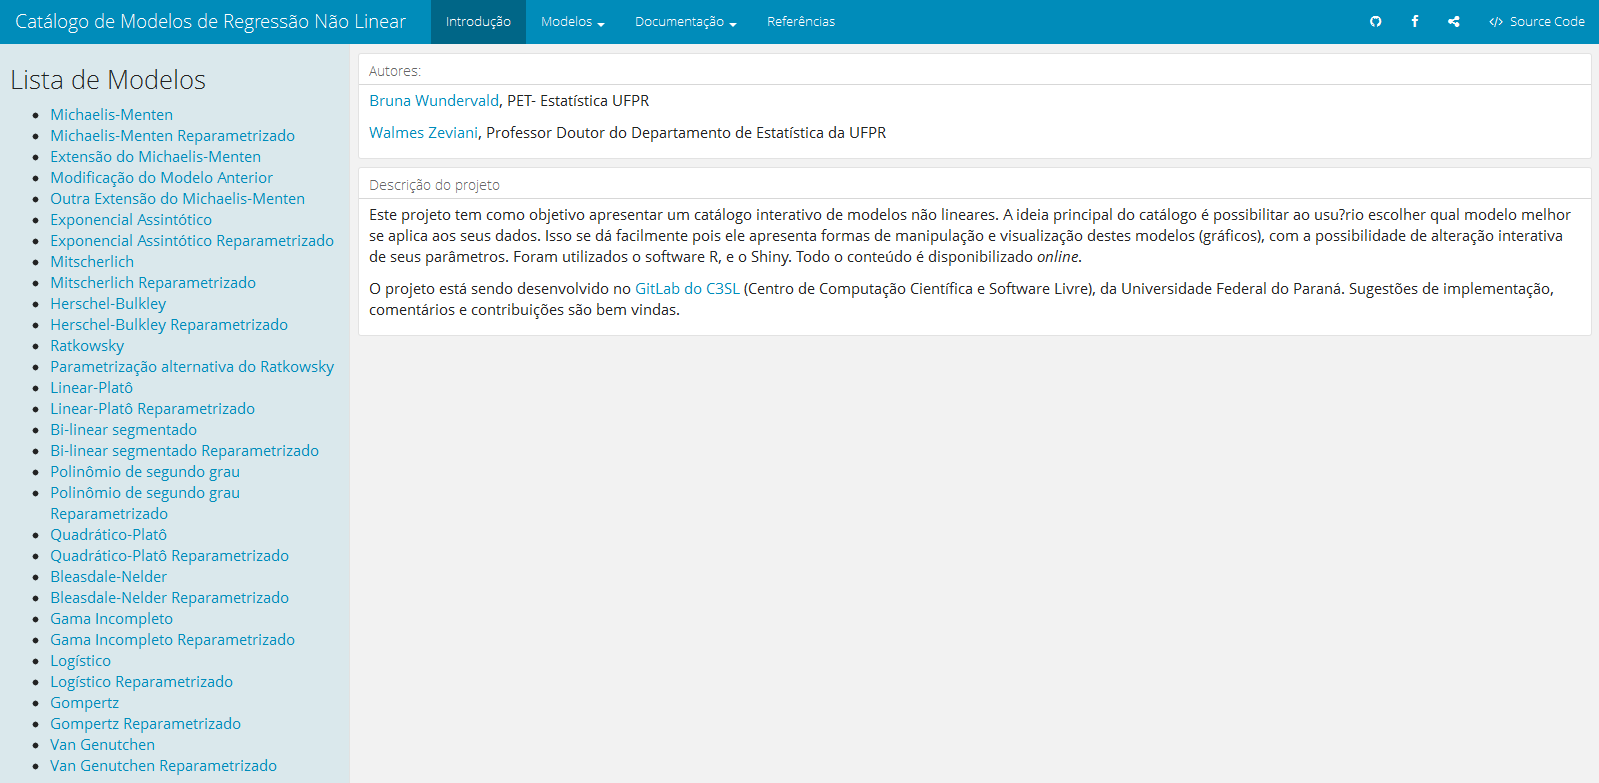
\includegraphics[width=\textwidth,height=1\textheight]{/home/bruna/GIT/pesqInd/prints/11.png}

\end{frame}

\begin{frame}


\includegraphics[height = .585cm]{/home/bruna/GIT/pesqInd/prints/2.png}


\includegraphics[width = 4cm]{/home/bruna/GIT/pesqInd/prints/3.png}

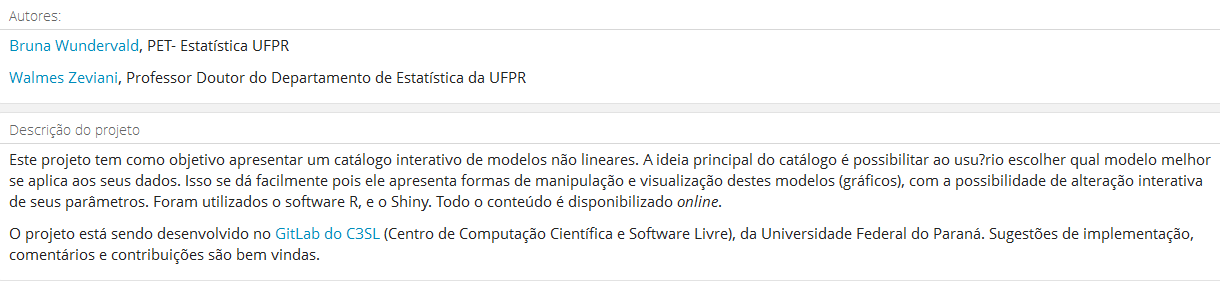
\includegraphics[width=\textwidth,height=0.5\textheight]{/home/bruna/GIT/pesqInd/prints/4.png}

\end{frame}

\begin{frame}

\vspace{-.3cm}\begin{columns}
 \begin{column}{.5\textwidth}

  \begin{center}
   \includegraphics*[height = 7.5cm]{/home/bruna/GIT/pesqInd/prints/1.png}
  \end{center}

 \end{column}
 \begin{column}{.5\textwidth}

  \begin{center}
   \includegraphics*[height = 7.5cm]{/home/bruna/GIT/pesqInd/prints/5.png}
  \end{center}

 \end{column}
\end{columns}

\end{frame}

\begin{frame}

\begin{columns}
 \begin{column}{.3\textwidth}

  \begin{center}
   \includegraphics*[height = 4.5cm]{/home/bruna/GIT/pesqInd/prints/6.png}
  \end{center}

 \end{column}
 \begin{column}{.7\textwidth}

  \begin{center}
   \includegraphics*[height = 6cm]{/home/bruna/GIT/pesqInd/prints/7.png}
  \end{center}

 \end{column}
\end{columns}

\end{frame}

\begin{frame}

\begin{center}
 \includegraphics*[width = 11.25cm, height = 5.2cm]{/home/bruna/GIT/pesqInd/prints/8.png}
\end{center}

\end{frame}

\begin{frame}

\vspace{-.15cm}\begin{center}
 \includegraphics*[width = 11.25cm, height = 6.5cm]{/home/bruna/GIT/pesqInd/prints/9.png}
\end{center}

\end{frame}

\begin{frame}

\vspace{-.25cm}\begin{center}
 \includegraphics*[height = 7cm]{/home/bruna/GIT/pesqInd/prints/12.png}
\end{center}

\end{frame}

\section{Resultados}\label{resultados}

\begin{frame}

\begin{itemize}
\tightlist
\item
  Melhoria geral na visualização dos modelos.
\item
  Disponibilização de uma coleção de visualização rápida de modelos, que
  ainda não existe sequer para as distribuições estatísticas mais
  comuns.
\item
  A interatividade permite maior compreensão e acertividade ao escolher
  um modelo.
\item
  Facilitação da compreensão de como eles funcionam.
\item
  Aprimoramento também da habilidade de visualizar equações que não
  estarão presentes no catálogo.
\end{itemize}

\end{frame}

\section{Pŕoximos Passos}\label{proximos-passos}

\begin{frame}

\begin{itemize}
\tightlist
\item
  Apresentar o Catálogo em conferências científicas de Estatística.
\item
  Construir aplicativos no mesmo formato com outros assuntos. Exemplo:
  \emph{Catálogo de Distribuições de Probabilidade}.
\item
  Gerar um módulo que permita o uso do catálogo de forma \emph{offline}.
\end{itemize}

\end{frame}

\section{Agradecimentos}\label{agradecimentos}

\begin{frame}

\begin{itemize}
\tightlist
\item
  C3SL - Centro de Computação Científica de Software Livre, da UFPR,
  pela disponibilização do GitLab.
\item
  LEG - Laboratório de Estatística e Geoinformação, pela
  disponibilização do servidor Shiny.
\end{itemize}

\end{frame}

\begin{frame}

\begin{center}

\Huge Obrigada pela atenção!

\vspace{0.5cm}

\includegraphics[width=.35\textwidth,height=.35\textheight]{/home/bruna/GIT/pesqInd/Pres/Prints/logo.png}

\end{center}

\end{frame}
